\documentclass{standalone}
\usepackage{tikz}
\usetikzlibrary{intersections}
\renewcommand{\familydefault}{\sfdefault}

\begin{document}
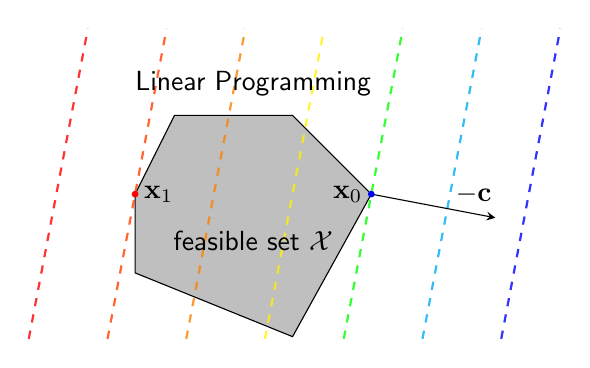
\begin{tikzpicture}[>=stealth]
%   \draw [fill = blue, opacity = .3] plot [smooth cycle] coordinates {(0,0) (1,1) (2,1) (3,-1) (0,-1)};
%   \draw [fill = red, opacity = .3] plot [smooth cycle] coordinates {(2,0) (3,2) (4, 1.5) (4, -1)};
%   \draw [fill = green, opacity = .3] plot [smooth cycle] coordinates {(1,2) (3,.3) (0, .1)};

%   \draw plot [smooth cycle] coordinates {(0,0) (1,1) (2,1) (3,-1) (0,-1)};
%   \draw  plot [smooth cycle] coordinates {(2,0) (3,2) (4, 1.5) (4, -1)};
%   \draw  plot [smooth cycle] coordinates {(1,2) (3,.3) (0, .1)};

  \begin{scope}[xshift = 6cm]
  \draw [fill = gray!50] (0, 0) -- (2, -.81) -- (3, 1) -- (2, 2) -- (.5, 2) -- (0, 1) -- cycle;
  
  \def\k{5.25}
  \def\ax{2.65}
  \def\bx{3.4}
  \def\ay{\d*(\ax - 3) + 1}
  \draw [thick, dashed, opacity = .8, green] ({\ax}, {\k*(\ax - 3) + 1}) -- ({\bx}, {\k*(\bx - 3) + 1});
  \draw [thick, dashed, opacity = .8, cyan] ({\ax +1}, {\k*(\ax - 3) + 1}) -- ({\bx+1}, {\k*(\bx - 3) + 1});
  \draw [thick, dashed, opacity = .8, blue] ({\ax +2}, {\k*(\ax - 3) + 1}) -- ({\bx+2}, {\k*(\bx - 3) + 1});
  \draw [thick, dashed, opacity = .8, yellow] ({\ax - 1}, {\k*(\ax - 3) + 1}) -- ({\bx-1}, {\k*(\bx - 3) + 1});
  \draw [thick, dashed, opacity = .8, orange] ({\ax - 2}, {\k*(\ax - 3) + 1}) -- ({\bx-2}, {\k*(\bx - 3) + 1});
  \draw [thick, dashed, opacity = .8, red!50!orange] ({\ax - 3}, {\k*(\ax - 3) + 1}) -- ({\bx-3}, {\k*(\bx - 3) + 1});
  \draw [thick, dashed, opacity = .8, red] ({\ax - 4}, {\k*(\ax - 3) + 1}) -- ({\bx-4}, {\k*(\bx - 3) + 1});
  \draw [->] (3, 1) -- (3 + .3*\k, 1 - .3);

  \draw [fill = blue, draw = blue] (3, 1 ) circle (1pt);
  \draw [fill = red, draw = red] (0, 1 ) circle (1pt);

  \node at (1.5, 0.4) {feasible set $\mathcal{X}$};
  \node at (1.5, 2.4) {Linear Programming};
  \node at (2.7, 1) {$\mathbf{x}_0$};
  \node at (.3, 1) {$\mathbf{x}_1$};
  \node at (4.3, 1) {$-\mathbf{c}$};
  % \draw (-1, .5) -- (3, -1.5);
  % \draw (1.5, -2) -- (3.5, 2);
  % \draw (-.5, .75) -- (3, 2.5);
  % \draw (0, -1) -- (0, 2);
  % \draw (3.5, .5) -- (1.5, 2.5);

  \end{scope}
\end{tikzpicture}
\end{document} 